\section{Representation of concepts on the Semantic Web}
\label{s:repr}

In this section we dive deeper into the semantics of RDF knowledge bases, attempting to make an (at least, approximate) dividing line not only between syntactic \textit{individuals} and \textit{classes} (as distinguished from the logics point of view), but also between ontological \textit{particulars} and \textit{universals}.
While this is not crucial for the execution of code list extraction presented in the previous two sections, we believe it can provide a broader context and help articulate the limitations of the presented approach and opportunities for extending it further.

When speaking about concepts, we will from now on specifically target `something that can be instantiated'.
Furthermore, we will assume that concepts can be instantiated by objects rather than by relationships.
Such a view of concepts is compatible with the notion of `concept' used as technical terms in the description logics (DL) underlying the Semantic Web, although, as we will see an ontological concept (universal) may often be meta-modeled by a surface individual (and thus be also understood as a non-instantiable individual from the DL point of view).

We hypothesized at the onset of our study described in Section~\ref{s:codelistanalyzer} that code list individuals would be more likely to represent ontological universals than ontological particulars.
By our manual analysis of extracted codes (Section~\ref{s:manual}), we identified that their majority corresponds to universals.\footnote{Since the universal/particular distinction is somewhat subtle, and given the relatively large size of the dataset examined, we do not provide a precise quantification; however, the estimated lower bound of the proportion of unarguable universals among the items judged as true codes was above 80 \%.} 
The only exceptions seem to be codes corresponding to qualities (such as colors), to entities whose universal/particular status is ambivalent (such as musical notes, which can refer either to individual symbols or to collections of `physical' notes having the same pitch), and only a few entities that look like genuine particulars (such as individual organizations). 

The prevalence of universals would probably be less obvious for knowledge graph individuals: considering the most prominent KGs, whether public or corporate ones, they are largely derived from Wikipedia articles.
Such articles may naturally refer to either universals (categories of entities such as biological taxa or occupational positions) or particulars (individual entities such as people, organizations or locations).
However, as one can easily check, e.g., through the `Random Article' link in Wikipedia, universals are only a minority in these resources -- this holds even if we consider `multi-copy' artifacts such as books or concrete consumer products to be universals. 

The rest of this section outlines a framework for studying the modeling of concepts (universals)  within the three types of knowledge bases -- ontologies, code lists, and knowledge graphs.
% -- characterized in Section~\ref{sections/02-structural-parts}. 
While only a part of the framework is directly related to the central task of detecting, extracting, and analyzing existing \emph{code lists} embedded in ontologies, the whole of it can help shed light on the follow-up opportunities of ensuring interoperability between concept collections in three kinds of knowledge bases.

\begin{table*}[pt]
\centering
\begin{tabular}{|P{3.6cm}|P{3.6cm}|P{3.6cm}|P{3.6cm}|}
\hline
\textbf{}                                        & \textbf{Ontology class}                                                                                         & \makecell{\textbf{Embedded code list}\\ \textbf{individual}}                                                & \textbf{KG individual}                                                                                                                                                                                                            \\ \hline
Concept representation                           & class                                                                                                           & individual                                                                  & individual                                                                                                                                                                                                                        \\ \hline
Meta-concept representation                      & \textit{rdfs:Class} (or, sometimes, \textit{owl:Class})                                                                           & OWL class, typically with a characteristic label (e.g., ending with ``Type'' & ontology class, or another individual                                                                                                                                                                                             \\ \hline
Linking to meta-concept                          & \textit{rdf:type}                                                                                                        & \textit{rdf:type                         }                                           & \textit{rdf:type}, or an arbitrary property                                                                                                                                                                                                \\ \hline
Instance representation                          & individual                                                                                                      & NONE                                                  & individual                                                                                                                                                                                                                        \\ \hline
Linking from instances                           & \textit{rdf:type}                                                                                                        & NONE                                                & arbitrary property                                                                                                                                                                                                                \\ \hline
Linking to super-concept/s and from sub-concepts & \textit{rdfs:subClassOf}                                                                                                 & \textit{skos:broader}, or often NONE                                                 & from sub-concepts: ad hoc object properties; to super-concepts modeled as KG individuals: ad hoc object properties; to super-concepts modeled as ontology classes: \textit{rdf:type} \\ \hline
Assignment properties                           & punning needed; possibly multiple properties with varying semantics                                    & usually just one property per code list                                      & possibly multiple properties                                                                                                                                                                                                      \\ \hline
Concept/s maintenance   & concept valid for the given version of the ontology; old concept may be kept with a `deprecated' annotation 
& concept valid for the given version of the ontology, together with the code list class     & irregular, often the validity period cannot be established, even when analyzing external resources                                                                                                                                       \\ \hline


\end{tabular}

  \caption{Comparison of three expected ways of representing concepts}
  \label{tab:comparison}
\end{table*}


\subsection{Generic template}
\label{ss:template}

In the template structure diagram Figure~\ref{fig:conc_diag_templ} we see the `focal' concept placeholder in the middle, surrounded with its structural context.
Above it is its \emph{meta-concept} (which the `focal' concept instantiates), and below it is its own \emph{instance}.
On its left-hand side is its \emph{super-concept}, as the concept that contains a (usually, proper) super-set of its instances, and analogously for the \emph{sub-concept} on the right-hand side of the `focal' concept.
Finally, there is an incoming edge from the right, referencing what we will label as \emph{assignment property}: a property that takes the concept as its value.


\begin{figure}[h]
\centering
%\captionsetup{justification=centering}
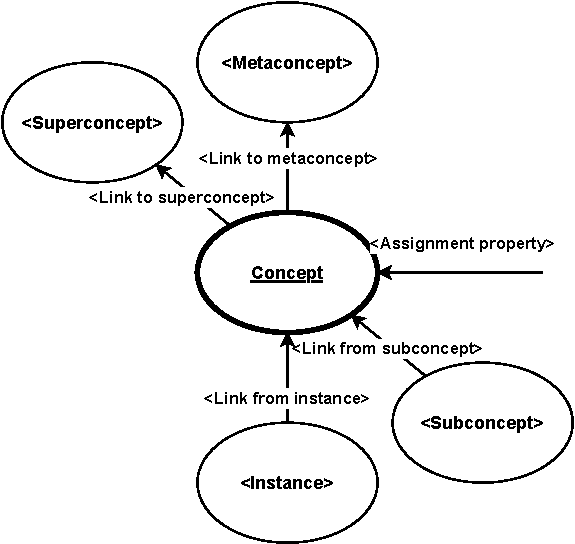
\includegraphics[width=7cm]{figures/conc_diag_templ.pdf}
\caption{Generic template structure}
\label{fig:conc_diag_templ}
%\vspace{-2mm}
\end{figure}

In this respect, note that assigning a concept as a property value is not quite obvious, neither from the formal point of view (specifically, if the concept is represented as an ontological class and not meta-modeled as an individual, whether a code list or knowledge graph one) nor from the semantic point of view.
    The formal compatibility issue was analyzed in the `Classes as Property Values' W3C note \cite{CPV}, on the example of assigning a book the class Lion as its subject (the assignment property being \emph{dc:subject} from the Dublin Core vocabulary), and later partially solved by \emph{punning} (already mentioned in Section~\ref{ss:def_type}) being allowed in OWL 2: the individual assigned by the property and the class share the same IRI, but are distinct in the logical space.
The semantic part of the issue was later scrutinized in a study \cite{KCap13} yielding three\footnote{For practical purposes, their numbering in this paper differs from the order in which they are introduced in the old study \cite{KCap13}.} different semantic motivations for `using a class as a property value', yielding three variants (V1--V3) depending on what aspect of the concept is actually to be valued by the property: 
\begin{itemize}
    \item \textbf{V1} the \emph{intension} of the concept, i.e., truly the concept as such;
    \item \textbf{V2} the \emph{extension} of the concept, i.e., the (sub)set of its instances (say, the set of all lions, some particular named lions, or a `prototypical' lion, in the book subject example);
    \item \textbf{V3}  an abstract \emph{topic} (being not a `canonical' universal, as its instantiation is an arguable matter) merely derived from the concept; e.g., a book has as subject the topic of lions rather than the concept of a lion.
    \end{itemize}
Looking at the first variant, we can still formulate some likely sub-variants for it: 
\begin{itemize}
    \item \textbf{V1a} The property is a `hooded' \emph{instantiation}, merely expressed by a custom property -- say, \emph{ex:speciesOfExemplar} (assigning an animal to its species or another taxon), if we stick to the class Lion as property value -- than by \emph{rdf:type}. Such a property is then not truly an assignment property but provides linking from instances, with respect to our template structure.
    \item \textbf{V1b} The property is, in a way, an inverted meta-property of the concept -- e.g., \emph{ex:proposedAsTaxon}, linking a biologist to their invented and proposed taxa, in the biological setting (some less ancient taxon than Lion should probably be used as a real example here). 
\end{itemize}

Let us now go through the expected ways the template is instantiated with respect to our three different types of knowledge representation.
For each of them we characterize the expected template instantiation (i.e., what kind of entities is likely to appear in the context of an entity representing a concept) for each of the knowledge representations, in a table (Table~\ref{tab:comparison}), also showing an example diagram using the same layout as in the template diagram. 
Aside from the structural context, we could also consider other aspects of the concept representation and management. 
Here we consider one complex aspect, the maintenance of the concept, in time, characterized in the last row of Table~\ref{tab:comparison}.



\subsection{Concept as an OWL class}

Modeling a concept as a class is the approach in which the logical semantics interweaves most closely with the deeper ontological semantics.
The only meta-concept of a class is normally (under the DL semantics) the specific \emph{rdfs:Class} entity (sometimes non-canonically substituted by \emph{owl:Class}).
Linking from instances via \emph{rdf:type}, and to super-concepts and from sub-concepts via \emph{rdfs:subClassOf}, is quite an obvious option.
On the other hand, as explained in Section~\ref{ss:template}, the use of assignment properties is trickier and has to rely on punning.
As designers of ontologies meant for real adoption will likely not obscure them with punning, the assignment properties, if any, would probably belong to a separate namespace. 

As an example, see the class \emph{dbo:Stream}, from the DBpedia Ontology, in Figure~\ref{fig:conc_diag_class}. 
The diagram contains elements of the real context of this class in the ontology and instance knowledge graph.
The only exception is the artificially added assignment property \emph{ex:hasHabitat}, thus displayed in grey.
It is an example of the variant V2 from Section~\ref{ss:template}: some animal, say, fish, lives in particular (certainly not even all) instances of stream, and not in the `stream concept' itself.


\begin{figure}[h]
\centering
%\captionsetup{justification=centering}
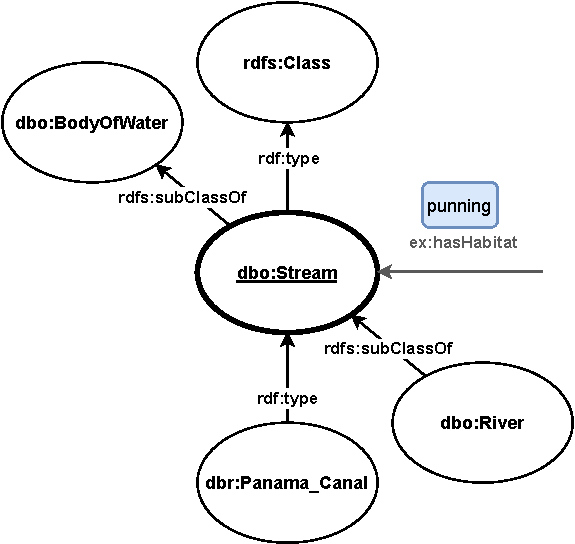
\includegraphics[width=7cm]{figures/conc_diag_class.pdf}
\caption{Class instance example from DBpedia}
\label{fig:conc_diag_class}
%\vspace{-2mm}
\end{figure}

As regards the maintenance of a class within an ontology, its complete replacement by another one is not common, since the curator of the ontology usually has no control on what and how many datasets already link to it; even if there is a new class with an altered definition, the old class is kept with an equivalence link to the new one (and with a `Deprecated' annotation label).
Furthermore, even if there may be closely related sets of sibling (or parent/child) classes, often such an update is applied on them individually.

%\medskip
%As we saw, there are many variations and subtle nuances of why and how concepts are modeled and linked in RDF knowledge bases.
%In the rest of the paper we will however confine ourselves to the situation from Figure~\ref{fig:conc_diag_c_ind}, where a code list is embedded in an ontology.


\begin{figure}[h]
\centering
%\captionsetup{justification=centering}
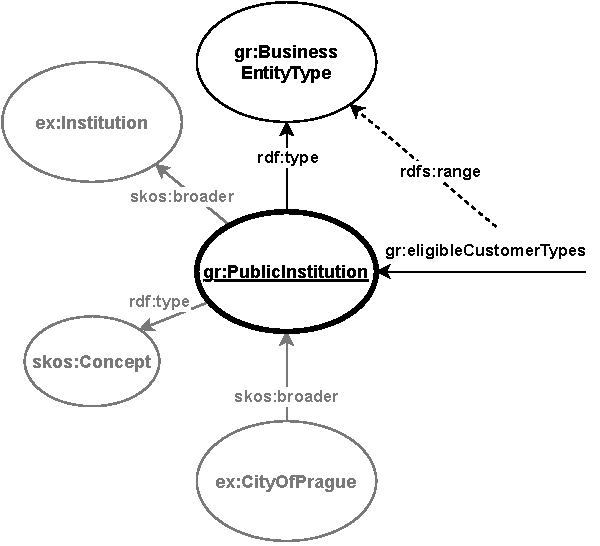
\includegraphics[width=7cm]{figures/conc_diag_c_ind}
\caption{Instance example from the GoodRelations ontology}
\label{fig:conc_diag_c_ind}
%\vspace{-2mm}
\end{figure}

\subsection{Concept as a code list individual}

%While the extraction of code lists in Section~\ref{s:codelistanalyzer} was entirely devoted to code lists embedded in ontologies, we will here review the expected setting covering even more stand-alone code lists, such as those primarily foreseen in the EU guidelines \cite{guide_code_list}.

First of all, the individual representing the concept will usually be linked via \emph{rdf:type} to a domain-specific class -- the \emph{code list class}.
The designers of the ontology often hint on the meta-modeling nature of this class by employing a naming convention: providing it with an ending such as ``-Type'' or ``-Kind''.
SKOS structures may be applied to express the links to super- and sub-concepts (\emph{skos:broader} and  \emph{skos:narrower}).
However, we would not expect to see linked instances: since the concept is modeled in the context of an ontology (within an embedded code list), if the designer wished to instantiate the given concept, s/he would have had the choice to express it as a class rather than as an individual.
The concept itself will then also be additionally typed as \emph{skos:Concept}, and linked to a SKOS concept scheme via \emph{skos:inScheme}.
For embedded code lists, it may typically be the case that they would be designed to serve a single assignment property, from the same namespace.
For standalone code lists with highly reusable codes (such as legal forms of organizations, or commodity types), linking via using multiple, independent, assignment properties is quite possible.

The example in Figure~\ref{fig:conc_diag_c_ind} shows the context of the \emph{gr:PublicInstitution} individual from the GoodRelations ontology \cite{GR}.
The individual is one of the four pre-defined individuals of the \emph{gr:BusinessEntityType} class (others are \emph{gr:Business}, \emph{gr:Enduser} and \emph{gr:Reseller}); note the naming pattern present in this (code list) class name.
SKOS is not referred to inside the whole GoodRelations specification; in the diagram, we however demonstrate its possible use (in grey), for better instructiveness.
There is however an assignment property, \emph{gr:eligibleCustomerTypes}.
It is the only property having \emph{gr:BusinessEntityType} as its range.
By the distinctions made in Section~\ref{ss:template}, the assignment of the concept by the property is, again, that of V2: individual public institutions (rather than the notion of a public institution) are eligible for a given business offer.


As regards maintenance, embedded code lists are likely to be updated with their code list classes as wholes, i.e., at irregular times.
Standalone code lists, such as those corresponding to RDF versions of official code lists used by government authorities \cite{DBLP:conf/smap/FilippidisKKIB16}, may, in turn, be updated regularly, e.g., annually.

\subsection{Concept as a knowledge graph individual}

Knowledge graphs are typically very large structures, powered by extractions from documents and/or large-scale crowdsourcing.
They have a natural propensity to model primarily via individuals, as it makes the graph simpler to handle.
These individuals are, in turn, secondarily endowed with links to classes from (typically, multiple) ontologies.
SKOS structures may sometimes be applied, namely, for portions of knowledge graphs that are inherent of hierarchical nature, such as category systems of underlying textual resources (the category system of Wikipedia, transferred to DBpedia, is a prominent example).
Knowledge graph concepts may have multiple independently created links to/from various context elements (in the sense of our framework).
As regards concept maintenance, individual knowledge graph concepts and links between them may often be updated in isolation, at arbitrary times (or, in knowledge graphs derived from textual resources such as Wikipedia, in arbitrary builds applied on these textual resources).

As a first example, in Figure~\ref{fig:conc_diag_kg_ind1}, we see the context of the \emph{dbc:Torpedo\_boats} individual from the DBpedia knowledge graph.
This individual is derived from the corresponding Wikipedia category.
Note that while the link from a sub-concept and that to the super-concept are defined via \emph{skos:broader}, the link from an instance and that to the super-class are defined via \emph{dct:subject}: a property that would not naturally be perceived as an analog of \emph{rdf:type} in the instance-to-instance setting.  
As the modeling derived from Wikipedia categories is inherently hierarchical, there are no properties that could be interpreted as assignment properties in terms of our framework.

\begin{figure}[h]
\centering
%\captionsetup{justification=centering}
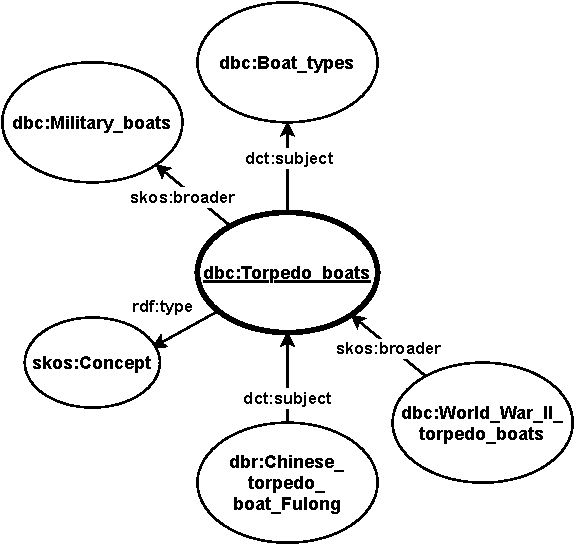
\includegraphics[width=7cm]{figures/conc_diag_kg_ind1.pdf}
\caption{Instance example from DBpedia}
\label{fig:conc_diag_kg_ind1}
%\vspace{-2mm}
\end{figure}

The second example, while also from DBpedia, is structurally completely different. 
In Figure~\ref{fig:conc_diag_kg_ind2} we see the context of the \emph{dbr:Wolverine} individual, which is a common resource derived from a Wikipedia page.
Note that \emph{rdf:type} is used here for the links both to a meta-concept and to a super-concept. 
This illustrates the common assumption that ontological cleanness is not always catered for in knowledge graphs.
As examples of assignment properties applied with the given concept, we show two.
If we look at them from the point of view of the distinctions from Section~\ref{ss:template}, the assignment of the concept by the property \emph{dbp:mascot} is likely a special kind of V2: the wolverine assigned (e.g., to some school) as mascot is not a real animal but a prototype one, yet, it is natural to view it as an instance of the wolverine concept.
The second property, \emph{dbp:shipNameSake}, in turn, rather falls under V1: if the \emph{name} of a ship is derived from the name of the biological genus, the assignment rather targets the intension of the concept.

\begin{figure}[ht]
\centering
%\captionsetup{justification=centering}
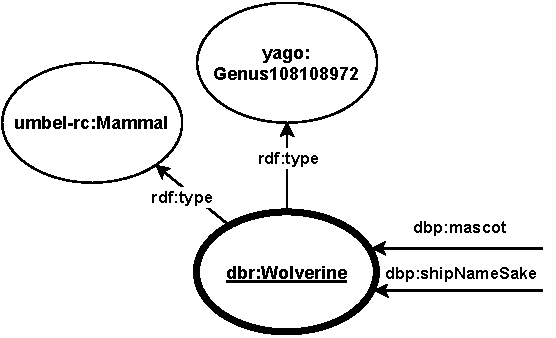
\includegraphics[width=7cm]{figures/conc_diag_kg_ind2.pdf}
\caption{Instance example from DBpedia with assignment properties}
\label{fig:conc_diag_kg_ind2}
%\vspace{-2mm}
\end{figure}
